\documentclass[11pt]{article}
\usepackage[T1]{fontenc}
\usepackage{lmodern,microtype,amsmath,amssymb,amsthm,mathtools,booktabs,array,xurl}
\usepackage[a4paper,margin=28mm]{geometry}
\usepackage{tikz}
\usetikzlibrary{arrows.meta,calc,positioning,intersections}
\usepackage[colorlinks=true,linkcolor=blue!55!black,citecolor=blue!55!black,urlcolor=blue!55!black]{hyperref}
\numberwithin{equation}{section}
\setlength{\emergencystretch}{2em}
\newtheorem{theorem}{Theorem}[section]
\newtheorem{proposition}[theorem]{Proposition}
\newtheorem{lemma}[theorem]{Lemma}
\newtheorem{corollary}[theorem]{Corollary}
\theoremstyle{definition}\newtheorem{definition}[theorem]{Definition}
\theoremstyle{remark}\newtheorem{remark}[theorem]{Remark}
\newcommand{\ii}{\mathrm i}
\newcommand{\dd}{\mathrm d}
\newcommand{\Vol}{\operatorname{Vol}}
\newcommand{\Turn}{\mathsf T}
\newcommand{\CC}{\mathbb C}
\newcommand{\RR}{\mathbb R}
\newcommand{\eps}{\varepsilon}
\newcommand{\kap}{\varkappa}
\title{Pyramids, prisms, and complete geometry\\of Conway closures}
\author{}\date{}
\begin{document}
\maketitle
\begin{abstract}
We construct the complete hyperbolic metric of an augmented link
specified by a completed Conway expression with two completed closing
children. A strict stationary point of its positive Newton source
determines ideal quadrangular pyramids and triangular prisms.
Stationarity matches their entire ordered quadrilateral faces.
We prove convexity throughout the assembly and identify the final
colored boundary with the literal projection cut of the original
diagram. Explicit face maps give the complete edge returns, including
the half-twist partners, and a common horocycle decoration proves cusp
completeness. The volume is twice the sum of the cell volumes, hence
$2\pi$ times the stationary source action. We also compute the primitive
crossing-circle lattice and give a constructive choice of half twists
for which the main strands form a knot. No assertion about signed
filling asymptotics or a nearby deformation is needed.
\end{abstract}

\section{The diagrams, the action, and the geometric theorem}
\label{cg:intro}

A crossing circle surrounds two strands and bounds a disk punctured
twice by them. The augmented diagram retains this circle and removes
full twists from the two strands. A retained half twist changes the
identification of the two sides of the disk. Throughout this paper the
disk, the endpoint order and the embedding of the whole construction
in the projection sphere are part of the data.

Label the four endpoints of a two-string box in cyclic order by
$0,1,2,3$, starting at the bottom left and moving to the bottom right.
For a stack $FG$, with $F$ below $G$, join $F_2$ to $G_1$ and $F_3$
to $G_0$. Its exposed tuple is $(F_0,F_1,G_2,G_3)$.
A clockwise quarter-turn moves the entire box and replaces its tuple
by $(F_1,F_2,F_3,F_0)$. Cylindrical closure joins the exposed endpoints
$0$ to $3$ and $1$ to $2$. These are physical operations on the
diagram, including all crossing disks.

\begin{definition}\label{cg:grammar}
Let $h$ be the quarter-turn of the elementary crossing-circle tangle,
with no retained twist. A completed expression is generated by
\[
 E::=hh\mid\Turn(E)\mid E_1E_2\mid hE\mid Eh.
\]
A closed expression is $C(FG)$, where both $F$ and $G$ are completed.
Every occurrence of $h$ is a distinct crossing circle.
\end{definition}

This is Definition~2.1 of \cite{Newton}. The adjective completed
specifies a rule for the expression, rather than a conclusion about
a metric. A single bare leaf at a closing child is outside the rule.
Write $H$ for the number of leaves.
Choose $\eps_\ell\in\{-1,0,1\}$ at each leaf. The augmented link
$L^\eps_E$ retains the indicated half twist and all its crossing
circles; put $Y^\eps_E=S^3\setminus L^\eps_E$. At this stage the main
strands may have several components.

\begin{figure}[ht]
\centering% Ordered boundary connections; boxes suppress their interior tangles.
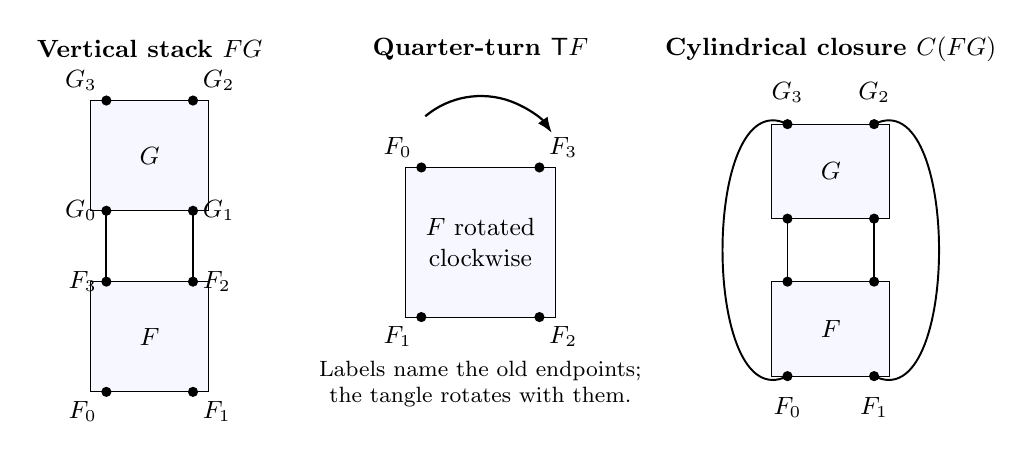
\begin{tikzpicture}[x=1cm,y=1cm, every node/.style={font=\small},
 tangent/.style={line width=.7pt}, terminal/.style={circle,fill=black,inner sep=1.3pt}]
% Left: stacking.
\begin{scope}[shift={(0,0)}]
 \node[font=\small\bfseries] at (1.2,4.8) {Vertical stack $FG$};
 \draw[fill=blue!3] (.45,.45) rectangle (1.95,1.85);
 \draw[fill=blue!3] (.45,2.75) rectangle (1.95,4.15);
 \node at (1.2,1.15) {$F$}; \node at (1.2,3.45) {$G$};
 \foreach \x in {.65,1.75} {
  \draw[tangent] (\x,1.85)--(\x,2.75);
  \foreach \y in {.45,1.85,2.75,4.15} \node[terminal] at (\x,\y) {};
 }
 \node[below left] at (.65,.45) {$F_0$};\node[below right] at (1.75,.45) {$F_1$};
 \node[left] at (.65,1.85) {$F_3$};\node[right] at (1.75,1.85) {$F_2$};
 \node[left] at (.65,2.75) {$G_0$};\node[right] at (1.75,2.75) {$G_1$};
 \node[above left] at (.65,4.15) {$G_3$};\node[above right] at (1.75,4.15) {$G_2$};
\end{scope}
% Middle: a genuine clockwise turn, showing old labels in new positions.
\begin{scope}[shift={(4.25,0)}]
 \node[font=\small\bfseries] at (1.15,4.8) {Quarter-turn $\mathsf T F$};
 \draw[fill=blue!3] (.2,1.4) rectangle (2.1,3.3);
 \node[align=center] at (1.15,2.35) {$F$ rotated\\clockwise};
 \foreach \p in {(.4,1.4),(1.9,1.4),(1.9,3.3),(.4,3.3)} \node[terminal] at \p {};
 \node[below left] at (.4,1.4) {$F_1$};\node[below right] at (1.9,1.4) {$F_2$};
 \node[above right] at (1.9,3.3) {$F_3$};\node[above left] at (.4,3.3) {$F_0$};
 \draw[-{Latex[length=2mm]},thick] (.45,3.95) arc[start angle=130,end angle=35,radius=1.1];
 \node[align=center,font=\footnotesize] at (1.15,.55) {Labels name the old endpoints;\\the tangle rotates with them.};
\end{scope}
% Right: closure arcs are actual identity connections outside both boxes.
\begin{scope}[shift={(8.65,0)}]
 \node[font=\small\bfseries] at (1.2,4.8) {Cylindrical closure $C(FG)$};
 \draw[fill=blue!3] (.45,.65) rectangle (1.95,1.85);
 \draw[fill=blue!3] (.45,2.65) rectangle (1.95,3.85);
 \node at (1.2,1.25) {$F$};\node at (1.2,3.25) {$G$};
 \foreach \x in {.65,1.75} {
  \draw[tangent] (\x,1.85)--(\x,2.65);
  \foreach \y in {.65,1.85,2.65,3.85} \node[terminal] at (\x,\y) {};
 }
 \draw[tangent] (.65,.65)..controls(-.45,.1)and(-.45,4.4)..(.65,3.85);
 \draw[tangent] (1.75,.65)..controls(2.85,.1)and(2.85,4.4)..(1.75,3.85);
 \node[below] at (.65,.5) {$F_0$};\node[below] at (1.75,.5) {$F_1$};
 \node[above] at (.65,4.0) {$G_3$};\node[above] at (1.75,4.0) {$G_2$};
\end{scope}
\end{tikzpicture}

\caption{The ordered stack, physical clockwise turn and cylindrical
closure. The label of an exposed endpoint is transported with its
box. The two connections inside a stack and the two outside closing
arcs are retained in the topological identification.}
\label{cg:fig-operations}
\end{figure}

We recall the real action with its normalization. Put
\[
 J(t)=\int_0^t\log(2\sin\pi u)\,\dd u,\qquad 0\le t\le1,
 \qquad J(1-t)=-J(t).
\]
The leaf and product functions are
\begin{align}
 g(a)&=-2J(a)-2J(1/2-a)=J(2a)-4J(a),\label{cg:g}\\
 m(x,y,z)&=J(x+y)+J(z)-J(x)-J(y)-J(z-x)\notag\\
 &\hspace{19mm}-J(z-y)-J(x+y-z).\label{cg:m}
\end{align}
A leaf has $0<a<1/2$. A strict product has
\begin{equation}\label{cg:strict}
 \max(x,y)<z<x+y<1,\qquad x,y>0.
\end{equation}
It is useful to write
\begin{equation}\label{cg:pqrw}
 p=z-x,\quad q=z-y,\quad r=x+y-z,\quad w=1-x-y.
\end{equation}
All four numbers are positive, and
\[
 p+q+2r+w=1,\quad x=q+r,\quad y=p+r,\quad 1-z=r+w.
\]
A physical turn replaces an output parameter $b$ by $1-b$.
At cylindrical closure the two outputs are $b$ and $1-b$.
The closing gate has been eliminated using that relation; it is not
an additional volume term. The action $\mathcal F$ is the sum of
$g$ over leaves and $m$ over product vertices on the resulting
polytope. Write $F_0$ for its maximum.

The precise variational input is as follows.
Proposition~5.3 of \cite{Newton} proves that $F_0$ is attained
at a unique strict point and that its Hessian in the free wire
coordinates is negative definite. It also proves that the fixed-output
profile $f_E(b)$ of a completed box is real analytic for $0<b<1$.
The profile maximizes over its internal wires, so the envelope
rule computes its derivative from its last cell. Lemma~6.1
of \cite{Newton} gives, at the closed maximum,
\begin{equation}\label{cg:leaf-window}
 \frac14<a_\ell<\frac{\arctan2}{\pi},
 \qquad \frac12<\cot(\pi a_\ell)<1 .
\end{equation}
Only the first two conclusions are needed to construct the metric.
The last will bound the crossing-circle shapes.

\begin{theorem}\label{cg:main}
For every fixed closed expression in Definition~\ref{cg:grammar}
and every choice of retained half twists $\eps$, the original exterior
$Y^\eps_E$ has a complete finite-volume hyperbolic metric. The metric
is assembled from two copies of a convex right-angled ideal
polyhedron, and
\begin{equation}\label{cg:volume}
 \Vol(Y^\eps_E)=2\pi F_0.
\end{equation}
At the $\ell$th crossing circle the original meridian and disk longitude
are a primitive ordered basis. With the half-twist convention of
Section~\ref{cg:peripheral}, the longitude-to-meridian ratio is
\begin{equation}\label{cg:cusp-shape}
 \tau_{\ell,\eps}
 =\frac{2\ii c_\ell}{1-\eps_\ell\ii c_\ell},
 \qquad c_\ell=\cot(\pi a_\ell)\in(1/2,1).
\end{equation}
All main cusp ends are complete as well.
\end{theorem}

The conclusion identifies the complement of the specified diagram,
not just a manifold with the same cell counts. It requires no
hyperbolic polyhedron existence theorem or assertion about the
complete character variety. The ideal-tetrahedron volume formula is
the classical input recalled in Section~\ref{cg:cells}. The Newton
stationary-point theorem is the only imported
construction-specific existence result.

\begin{corollary}\label{cg:source-volume}
Let $Z_{F,G,N}$ be the pure complete auxiliary-color source of
\cite[Section~2]{Newton}, with each leaf evaluated as $h_N$ and no
retained half twist. It is strictly positive for all sufficiently
large $N$, and through all sufficiently large integer levels
\[
 \lim_{N\to\infty}\frac{2\pi}{N}\log Z_{F,G,N}
       =\Vol(Y^0_E)=\Vol(Y^\eps_E).
 \]
\end{corollary}
\begin{proof}
Corollary~5.4 of \cite{Newton} gives the limit $F_0$ before multiplying
by $2\pi$; Theorem~\ref{cg:main} identifies that number with the metric
volume. The scalar here is the pure positive source, not a signed
filled-knot invariant.
\end{proof}

The decomposition of fully augmented links into right-angled
polyhedra and the effect of half twists are established parts of
augmented-link geometry; see \cite{Purcell}. The relation between a
concave action and hyperbolic volume belongs to the variational
setting discussed by Rivin \cite{Rivin}. The task here is to identify
the particular stationary pyramids and prisms with the original
completed diagram, with all orders and peripheral markings retained.
We give that construction directly.

\section{The two hyperbolic cells}\label{cg:cells}

We work in upper half-space, with ideal boundary
$\CC\cup\{\infty\}$. A geodesic plane is vertical over a line or
is a hemisphere orthogonal to the boundary plane. A horosphere
centered at $\infty$ is horizontal; its induced metric is Euclidean
up to scale. An ideal tetrahedron with dihedral angles
$\pi a,\pi b,\pi c$ at an ideal vertex, where $a,b,c>0$ and
$a+b+c=1$, has volume
\begin{equation}\label{cg:tetra}
\begin{split}
 V(a,b,c)&=\Lambda(\pi a)+\Lambda(\pi b)+\Lambda(\pi c)
        =-\pi[J(a)+J(b)+J(c)],\\
 \Lambda(t)&=-\int_0^t\log(2\sin u)\,\dd u .
\end{split}
\end{equation}
This is the ideal-tetrahedron formula of \cite{Milnor}. Its
normalization, including its vanishing at a flat tetrahedron,
fixes the absolute volume used below.

\subsection{The elementary pyramid}
For a leaf parameter $a$, put $E=e^{2\pi\ii a}$ and take
\begin{equation}\label{cg:leaf-coordinates}
 O=\infty,\qquad (C_0,C_1,C_2,C_3)=(1,E,-1,-E).
\end{equation}
Their convex hull is an ideal quadrangular pyramid. The four finite
vertices form a rectangle, so the four edges incident to $O$ have
dihedral angle $\pi/2$. Its base is an ordered quadrilateral
gluing face. Call its edges $01,23$ free and $12,30$ cap edges.
The base angles are $\pi a$ at the free edges and
$\pi(1/2-a)$ at the cap edges. These follow by intersecting the
vertical side planes with the unit hemisphere, or by reading
the half-arcs of the unit circle.

Color $(O,C_1,C_2)$ and $(O,C_3,C_0)$ shaded.
The other two side triangles are white. Shaded faces will record
the sides of a half crossing disk; white faces will record
regions of the projection sphere. A base diagonal gives
two positive tetrahedra with angle triple $(a,1/2-a,1/2)$.
Consequently
\begin{equation}\label{cg:leaf-volume}
 \Vol(\text{pyramid})=2V(a,1/2-a,1/2)=\pi g(a).
\end{equation}
\begin{figure}[ht]
\centering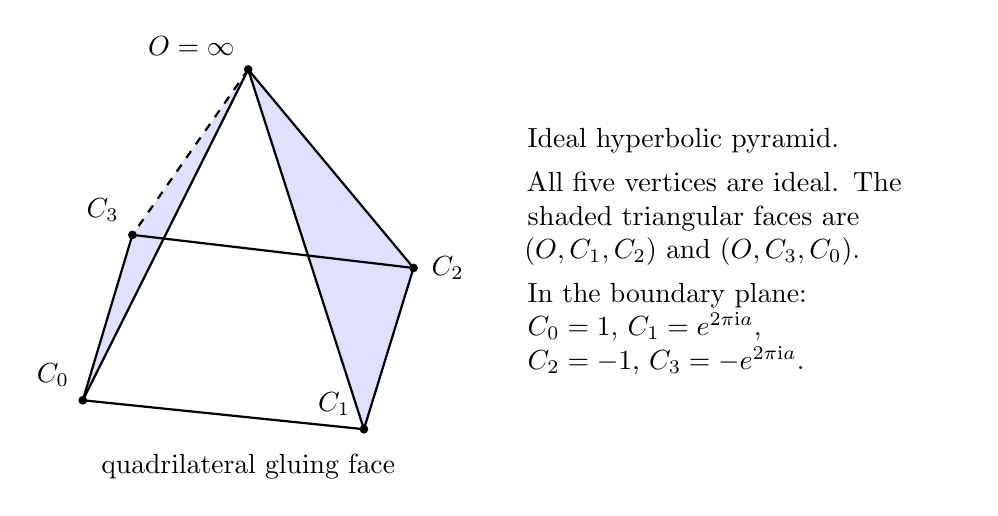
\begin{tikzpicture}[scale=1.05]
\coordinate (c0) at (-2,-1);\coordinate(c1) at (1.4,-1.35);\coordinate(c2) at (2,.6);\coordinate(c3) at (-1.4,1);\coordinate(o) at (0,3);
\fill[blue!12] (o)--(c1)--(c2)--cycle;\fill[blue!12] (o)--(c3)--(c0)--cycle;
\draw[thick] (c0)--(c1)--(c2)--(c3)--cycle;
\draw[thick] (o)--(c0) (o)--(c1) (o)--(c2);\draw[thick,dashed] (o)--(c3);
\foreach \p/\l in {c0/C_0,c1/C_1,c3/C_3,o/O=\infty}{\fill (\p) circle(1.5pt);\node[above left=2pt] at (\p) {$\l$};}
\fill (c2) circle(1.5pt);\node[right=3pt] at (c2) {$C_2$};
\node at (0,-1.8) {quadrilateral gluing face};
\node[align=left,text width=5.5cm] at (6,.8) {Ideal hyperbolic pyramid.\\[4pt]All five vertices are ideal. The shaded triangular faces are $(O,C_1,C_2)$ and $(O,C_3,C_0)$.\\[4pt]In the boundary plane:\\ $C_0=1$, $C_1=e^{2\pi\ii a}$,\\ $C_2=-1$, $C_3=-e^{2\pi\ii a}$.};
\end{tikzpicture}

\caption{The ideal hyperbolic pyramid of one leaf. The two shaded
triangles retain their labels throughout the construction.
The ordered quadrilateral base is auxiliary cut data, rather than
the four-punctured boundary of the physical tangle box.}
\label{cg:fig-leaf}
\end{figure}

\subsection{The multiplication prism}
Given a strict product, use \eqref{cg:pqrw} and put
\begin{equation}\label{cg:prism-vertices}
 v_0=1,\quad v_1=e^{2\pi\ii p},\quad
 v_2=e^{2\pi\ii(p+r)},\quad
 v_3=e^{2\pi\ii(p+r+q)} .
\end{equation}
The successive half-arcs are $p,r,q,r+w$. Let $P$ be the intersection
of $v_0v_1$ and $v_2v_3$. The triangle $(P,v_1,v_2)$ has
angles $\pi w,\pi y,\pi x$ at $P,v_1,v_2$, respectively.
The sine rule gives
\begin{equation}\label{cg:prism-P}
\begin{split}
 P&=v_1+\frac{\sin\pi x\sin\pi r}
                 {\sin\pi w\sin\pi p}(v_1-v_0)\\
  &=v_2+\frac{\sin\pi y\sin\pi r}
                 {\sin\pi w\sin\pi q}(v_2-v_3).
\end{split}
\end{equation}
Both coefficients are positive. Thus $P$ lies beyond $v_1$ from
$v_0$ and beyond $v_2$ from $v_3$, and $|P|>1$.

Start with the quadrangular pyramid
$(\infty,v_0,v_1,v_2,v_3)$ and attach
$(\infty,P,v_1,v_2)$ on the other side of their common triangle.
The faces over $v_0v_1$ and $Pv_1$ are coplanar, as are those over
$v_3v_2$ and $Pv_2$. After merging them the boundary consists of
two white triangles $(P,v_1,v_2)$ and $(\infty,v_0,v_3)$ and three
ordered quadrilaterals
\begin{equation}\label{cg:prism-faces}
 F_x=(\infty,v_0,v_1,P),\quad
 F_y=(\infty,v_3,v_2,P),\quad
 F_z=(v_0,v_1,v_2,v_3).
\end{equation}
The vertical supporting planes lie over $v_0v_1$, $v_2v_3$
and $v_3v_0$. The other two planes are the hemispheres through
$(v_0,v_1,v_2,v_3)$ and $(P,v_1,v_2)$. Formula
\eqref{cg:prism-P} puts $P$ outside the first boundary circle and
$v_0,v_3$ outside the second. Their inward half-spaces therefore
contain precisely the attached pieces. This proves that their union
is a convex ideal triangular prism.
\begin{figure}[ht]
\centering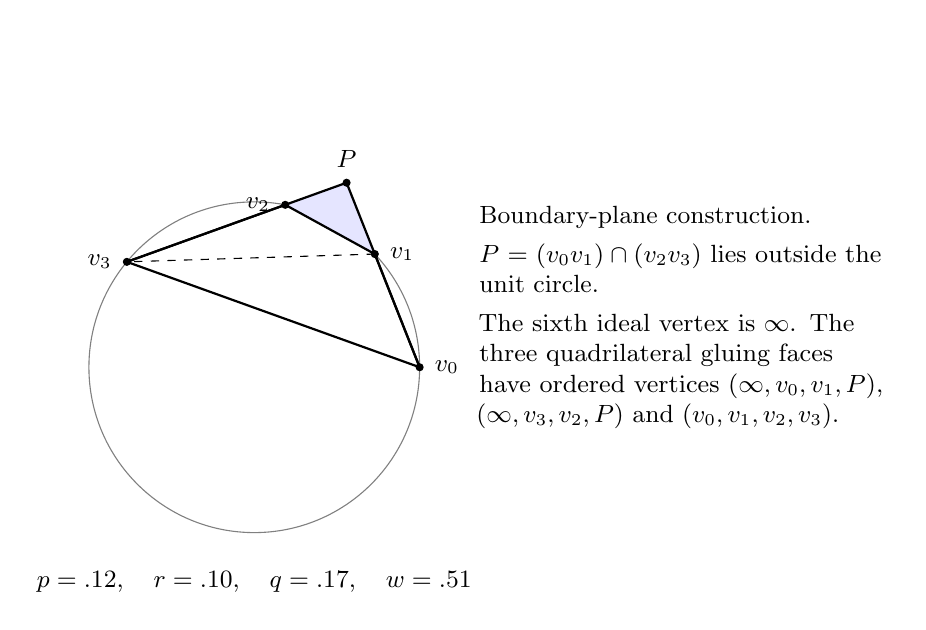
\begin{tikzpicture}[scale=2.1, every node/.style={font=\small}]
\coordinate(v0) at (1,0);
\coordinate(v1) at ({cos(43.2)},{sin(43.2)});
\coordinate(v2) at ({cos(79.2)},{sin(79.2)});
\coordinate(v3) at ({cos(140.4)},{sin(140.4)});
\coordinate(P) at (0.57935,1.06242);
% Exact intersection of the two extended chords is used below.
\path[name path=first] (v0)--($(v0)!3!(v1)$);
\path[name path=second] (v3)--($(v3)!3!(v2)$);
\path[name intersections={of=first and second,by=P}];
\draw[gray] (0,0) circle(1);
\fill[blue!10] (P)--(v1)--(v2)--cycle;
\draw[thick] (v0)--(P)--(v3)--cycle;
\draw[thick] (v0)--(v1)--(v2)--(v3);
\draw[dashed] (v1)--(v3);
\foreach \p/\lab/\pos in {v0/v_0/right,v1/v_1/right,v2/v_2/left,v3/v_3/left,P/P/above}
 {\fill (\p) circle(.7pt);\node[\pos=2pt] at(\p){$\lab$};}
\node at (0,-1.3) {$p=.12,\quad r=.10,\quad q=.17,\quad w=.51$};
\node[align=left,text width=5.2cm] at (2.6,.3) {Boundary-plane construction.\\[3pt]$P=(v_0v_1)\cap(v_2v_3)$ lies outside the unit circle.\\[3pt]The sixth ideal vertex is $\infty$. The three quadrilateral gluing faces have ordered vertices $(\infty,v_0,v_1,P)$, $(\infty,v_3,v_2,P)$ and $(v_0,v_1,v_2,v_3)$.};
\end{tikzpicture}

\caption{The boundary-plane support data for a multiplication prism.
The point $P$ is the exact intersection of the two extended chords;
the sixth ideal vertex is $\infty$. The example illustrates one
strict tuple. Formula \eqref{cg:prism-P} proves the construction
throughout \eqref{cg:strict}.}
\label{cg:fig-prism}
\end{figure}

The full dihedral-angle table is
\begin{center}
\begin{tabular}{lc}
\toprule Edges & Angle divided by $\pi$\\ \midrule
$Pv_1,\ \infty v_0$ & $x$\\
$Pv_2,\ \infty v_3$ & $y$\\
$v_1v_2,\ v_0v_3$ & $1-z$\\
$P\infty$ & $w$\\
$v_0v_1$ & $p$\\
$v_2v_3$ & $q$\\ \bottomrule
\end{tabular}
\end{center}
The first two rows are the angles of $(P,v_1,v_2)$ and their
opposite edges; the last two are half-arcs of the unit circle.
At each trivalent ideal vertex the interior dihedral angles sum
to $\pi$; for instance the three at $P$ sum to
$\pi(x+y+w)=\pi$.

Triangulate the quadrangular pyramid across $v_0v_2$. Its two
tetrahedra have triples $(p,r,1-p-r)$ and $(p+r,q,r+w)$.
The complementary terms with arguments $p+r$ and $1-p-r$ cancel
in \eqref{cg:tetra}. The remaining four Lobachevsky terms also
equal the sum for the two positive triples
$(p,q,2r+w)$ and $(p+q,r,r+w)$.
The attached tetrahedron has triple $(y,x,w)$. Hence
\begin{equation}\label{cg:prism-volume}
\begin{split}
 \Vol(\text{prism})
 &=V(y,x,w)+V(p,q,2r+w)+V(p+q,r,r+w)\\
 &=\pi m(x,y,z).
\end{split}
\end{equation}
All these triples are strictly positive and sum to one. The
equality is an ordinary sum of metric volumes.

\section{Ordered face matching and convex assembly}
\label{cg:assembly}

\subsection{The whole quadrilateral, including its shear}
For cyclically ordered points on a circle or line define
\begin{equation}\label{cg:kappa}
 \kap(a,b,c,d)=\frac{(a-b)(c-d)}{(a-d)(b-c)}>0,
\end{equation}
with limits at infinity. Sending three ordered vertices to
$(\infty,0,1)$ shows that $\kap$ determines the ordered ideal
quadrilateral up to isometry. It fixes its diagonal shear as well
as its labels. A one-step cyclic shift, or reversal fixing the
first vertex, inverts $\kap$. Full reversal
$(a,b,c,d)\mapsto(d,c,b,a)$ preserves it.

The prism coordinates give
\begin{align}
 \kap(F_x)&=\frac{\sin\pi x\sin\pi r}{\sin\pi w\sin\pi p}
              =e^{-m_x},&
 \kap(F_y)&=\frac{\sin\pi y\sin\pi r}{\sin\pi w\sin\pi q}
              =e^{-m_y},\label{cg:input-kappa}\\
 \kap(F_z)&=\frac{\sin\pi p\sin\pi q}{\sin\pi z\sin\pi r}
              =e^{-m_z}.&&\label{cg:output-kappa}
\end{align}
Differentiating \eqref{cg:g} gives the leaf formula
$\kap(C_0,C_1,C_2,C_3)=\tan^2(\pi a)=e^{-g'(a)}$.
For a product $FG$ the actual attachment maps are
\begin{equation}\label{cg:stack-maps}
\begin{array}{c|cccc}
 &C_0&C_1&C_2&C_3\\ \hline
 F&v_0&v_1&P&\infty\\
 G&\infty&P&v_2&v_3 .
\end{array}
\end{equation}
The first is a cyclic shift of $F_x$, and the second is reversal
fixing the first vertex of $F_y$. They invert the input value of
$\kap$. If $f_F$ is the stationary output profile of the lower
child, its wire equation is $f_F'(x)+m_x=0$; the upper equation
is the same with $G,y$. Thus the output and input values of
$\kap$ multiply to one, exactly the condition for the assignments
\eqref{cg:stack-maps} to extend to whole-face isometries.
The new profile has derivative $m_z$. This inductively proves
the output formula $\kap=e^{-f_E'}$.
A turn cyclically relabels the face and replaces $b$ by $1-b$,
which has the same reciprocal effect.

\subsection{Why successive attachments stay convex}
Local angle equations do not by themselves exclude overlap of
distant pieces. The following elementary argument controls the
whole union.

\begin{lemma}\label{cg:convex-union}
Place two finite ideal convex polyhedra on opposite sides of the
plane of an isometric maximal face. If every finite boundary seam
of their union has total interior angle at most $\pi$, the union
is convex. If the common face is a quadrilateral with strictly
nonflat boundary edges in each piece, their ideal closures have
no intersection other than the four recorded face vertices.
\end{lemma}
\begin{proof}
The finite part of the union is closed in hyperbolic space and
locally convex. At a seam edge this is exactly the angle condition;
away from a seam it follows from convexity of the pieces.
Any two finite points can be joined in the union by a finite-length
path. A minimizing sequence with bounded length stays in a compact
ambient hyperbolic ball. Constant-speed parametrization and a
uniformly convergent subsequence give a shortest path in the
union. Local convexity makes it an ambient geodesic near every
point. It is therefore the unique ambient segment, proving
convexity.

The opposite closed half-spaces meet only in their supporting plane.
Their ideal closures can meet only on its boundary circle.
The intersection of either polyhedron with that plane is exactly
its maximal face. An additional ideal vertex in the plane would
enlarge the face across a boundary edge and make that edge flat,
contrary to the strict hypothesis. In the Klein model the closure
of an ideal quadrilateral meets the sphere at infinity at precisely
its four vertices. This excludes every unrecorded ideal
intersection.
\end{proof}

An elementary output has free angle $\pi a$ and cap angle
$\pi(1/2-a)$. Inductively, a completed output $b$ has free angle
$\pi b$ and cap angle $\pi(1-b)$. Attach the lower child first.
At a cap seam a leaf gives total angle $\pi/2$, while a completed
child gives $\pi$ and joins two white faces. The edge shared by the
two prism inputs now has angle
$\pi(w+x)=\pi(1-y)<\pi$. Thus the other input remains a maximal
supported quadrilateral face. Lemma~\ref{cg:convex-union} applies
again when the upper child is attached. We have not assumed
nonintersection between two independently placed children.

The final common input edge has angle $\pi(w+x+y)=\pi$.
The free output seams have angles $\pi(p+x)=\pi z$ and
$\pi(q+y)=\pi z$; the cap output edges have angle $\pi(1-z)$.
Every remaining edge is an original shaded-triangle edge and is
right angled. Flat seams join white faces. Strictness of the
output parameter keeps its face maximal and supported, so the
induction continues.

There is a separate combinatorial check at ideal vertices.
At every open stage the four exposed corners are four unpaired
original terminal points. Product consumes the disjoint pairs
$F_2/G_1$ and $F_3/G_0$ and never exposes them again; a turn merely
permutes the unpaired points. Later identifications cannot extend
a consumed pair into a longer chain. Each final main vertex is
exactly a pair of original terminals, and a leaf's four corners
stay distinct. Its crossing-circle apex is not among those
terminals. Together with Lemma~\ref{cg:convex-union}, this shows
that every leaf retains two distinct shaded triangles sharing only
their original apex.

\subsection{Closing the two completed children}
At the root the outputs are $b,1-b$. The free root equation is
$f_F'(b)=f_G'(1-b)$, so their ordered quadrilaterals have the same
$\kap$. The closing map is
\begin{equation}\label{cg:root}
 C_j^F\longmapsto C_{3-j}^G,\qquad j\pmod4.
\end{equation}
Full reversal preserves $\kap$ and simultaneously realizes the
two stack connections and the two outside closing connections.
Each pair of free angles sums to $\pi$, as does each pair of cap
angles. The last gluing thus joins white faces across flat seams.
The result is a convex right-angled ideal polyhedron $P_E$, with
\begin{equation}\label{cg:half-volume}
 \Vol(P_E)=\pi\sum_\ell g(a_\ell)
             +\pi\sum_{\text{products}}m(x,y,z)=\pi F_0 .
\end{equation}
There are $2H$ shaded triangles, $3H$ ideal vertices and $6H$
edges; Euler's formula gives $H+2$ white faces. These counts are
consequences of the assembly. The next section identifies its
entire labeled boundary.

\section{Recovering the original cut balls}
\label{cg:topology}

Place the pure main strands in the projection sphere, retaining
the crossing disks in their disjoint elementary boxes. Cut the
link exterior along that sphere. Each auxiliary circle becomes
a semicircle in each projection ball, boundary-parallel along its
original half crossing disk. Drilling a boundary-parallel semicircle
introduces one handle; cutting along its half disk opens precisely
that handle. The half disks are disjoint, so these cancellations
can be performed successively in the original boxes. Each result
is a ball with ideal vertices. Main strand segments lie on its
boundary; their removal creates ideal corners and no interior
handles.

At a leaf the cut produces exactly
$(O,C_1,C_2)$ and $(O,C_3,C_0)$ as its shaded triangles.
The other faces are regions of the original projection sphere.
We determine their full walks as follows. At $O$ keep the cyclic
order $(C_0,C_1,C_2,C_3)$. At an outer corner each shaded triangle
contributes the sector ordered by its next and previous neighbors.
The identity strip joining two terminals concatenates their two
sectors in planar order. A boundary walk entering a vertex along
an oriented edge $(u,v)$ exits along the neighbor preceding $u$
in the cyclic order at $v$. Thus the shaded triangles and terminal
pairings determine every remaining white walk.

The maps \eqref{cg:stack-maps} identify $F_2$ with $G_1$ at $P$,
and $F_3$ with $G_0$ at $\infty$. Their exposed order is
$(F_0,F_1,G_2,G_3)=(v_0,v_1,v_2,v_3)$. The prism's two white
triangles insert exactly the intervening white sectors.
At a completed cap seam those sectors merge across a flat
white edge; at a leaf cap seam their boundary remains an original
shaded edge. Turns transport the cyclic order, and
\eqref{cg:root} realizes the original closing pairs. Hence the
ribbon orders of the final nonflat graph are the orders of the
literal projection cut. All faces, including every white walk,
have the same labels and cyclic orders.

This gives a label-preserving cellular homeomorphism of each
cut-ball boundary with $\partial P_E$. A sphere homeomorphism
extends over a ball, for example radially after choosing ball
coordinates. Gluing the two extended balls along their prescribed
white and shaded faces reverses exactly the original cuts.
The quotient is $Y^0_E$, with degree one and the original disk
curves retained.

An ordered quadrilateral during assembly is auxiliary cut data.
It is not the physical four-punctured boundary of the tangle box.
We first used its modulus to assemble cells, and then used the
closed ribbon identification to recover the physical complement.
No boundary group representation is inferred from quadrilateral
moduli alone.

For a retained half twist, cut the twice-punctured disk and rotate
one side through $\pi$. This interchanges both punctures and the
upper and lower half disks. The two balls and white faces are
unchanged. Superscripts distinguishing the projection copies give
the new shaded maps
\begin{equation}\label{cg:odd-pairing}
\begin{array}{c|ccc}
 S_0^+\longrightarrow S_1^-&O&C_1&C_2\\
                          &O&C_3&C_0\\ \hline
 S_1^+\longrightarrow S_0^-&O&C_3&C_0\\
                          &O&C_1&C_2 .
\end{array}
\end{equation}
The other maps are their inverses. Both signs give this unmarked
pairing; the original meridian paths differ, as computed in
Section~\ref{cg:peripheral}. The same labeled balls therefore give
the original $Y^\eps_E$.

\section{Entire face maps and edge returns}
\label{cg:maps}

The construction matches complete faces isometrically. We now
give the complex-coordinate dictionary for their identifications.
It records the shear and checks the entire edge return, including
translation. Matrices are projective, and composition acts from
right to left.

\subsection{The leaf and its adjacent white faces}
Normalize the ordered base of a leaf to $(0,\infty,1,R)$.
At completeness,
\begin{equation}\label{cg:normalized}
 E=e^{2\pi\ii a},\qquad Z=\frac{1+E}{2},\qquad
 R=\frac{(1+E)^2}{4E}=\cos^2(\pi a).
\end{equation}
The apices in the two charts are $Z$ and $Z/E=\overline Z$.
Their white or completion maps are
\begin{equation}\label{cg:white}
\begin{aligned}
 W_0&=\begin{pmatrix}1&0\\0&E\end{pmatrix},&
 W_1&=\begin{pmatrix}1&E-1\\0&E\end{pmatrix},\\
 W_2&=\begin{pmatrix}E-R&R(1-E)\\E-1&1-ER\end{pmatrix},&
 W_3&=\begin{pmatrix}R&0\\1-E&ER\end{pmatrix}.
\end{aligned}
\end{equation}
The elementary pyramid has actual white faces only at $W_0,W_2$.
The expressions $W_1,W_3$ describe the maps supplied by the
adjacent prism at its cap edges. This is proved below before
using them in a group word.

The pure within-copy shaded map and the odd cross-copy maps are
\begin{equation}\label{cg:shaded}
\begin{aligned}
 S&=\begin{pmatrix}0&-ER\\1&-1-E\end{pmatrix},&
 A&=\begin{pmatrix}R&-R\\1&ER-1-E\end{pmatrix},&
 B&=\begin{pmatrix}R/E-1-1/E&R\\-1&R\end{pmatrix}.
\end{aligned}
\end{equation}
Their vertex assignments are
\[
 S:(Z,\infty,1)\mapsto(Z,0,R),\quad
 A:(Z,\infty,1)\mapsto(Z/E,R,0),\quad
 B:(Z,R,0)\mapsto(Z/E,\infty,1).
\]
Three ordered vertices determine the maps; substitution of
$Z^2-(1+E)Z+ER=0$ verifies their apex values. At the complete
parameters all these matrices are invertible.

\subsection{Compatibility across an entire prism}
Use independent phase variables $\alpha,\beta,\gamma$ for
$e^{2\pi\ii p},e^{2\pi\ii r},e^{2\pi\ii q}$.
The world coordinates are
\begin{equation}\label{cg:phase-coordinates}
\begin{split}
 v_0&=1,\quad v_1=\alpha,\quad
 v_2=\alpha\beta,\quad v_3=\alpha\beta\gamma,\\
 P&=1+\alpha-
 \frac{\alpha[\alpha\beta(1+\gamma)-1-\alpha]}
             {\alpha^2\beta^2\gamma-\alpha}.
\end{split}
\end{equation}
Indeed the chord lines have equations
$P+\alpha\overline P=1+\alpha$ and
$P+\alpha^2\beta^2\gamma\overline P=\alpha\beta(1+\gamma)$,
which give \eqref{cg:phase-coordinates}.
For an ordered quadrilateral $(a,b,c,d)$ use
\[
 M_{a,b,c}(z)=\frac{(z-a)(c-b)}{(z-b)(c-a)},\qquad
 R=M_{a,b,c}(d).
\]
Its world white map is $\overline M^{-1}W_j(E,R)M$.
Here the bar reciprocates $\alpha,\beta,\gamma$; on the complete
unit-circle chamber it is complex conjugation.
For the lower, upper and output quadrilaterals in
\eqref{cg:stack-maps} and \eqref{cg:prism-faces}, their wire
phases are $\beta\gamma,\alpha\beta,\alpha\beta\gamma$.
In these common world coordinates the entire maps obey
\begin{equation}\label{cg:nine}
\begin{aligned}
 W_{F,1}=W_{G,1}=W_{o,1}&=W_{\rm top},&
 W_{F,3}=W_{G,3}=W_{o,3}&=W_{\rm bottom},\\
 W_{F,2}&=W_{G,0},&
 W_{o,0}=W_{F,0},\qquad W_{o,2}&=W_{G,2}.
\end{aligned}
\end{equation}
The subscript $o$ means output. The top and bottom maps take
$(P,v_1,v_2)$ and $(\infty,v_0,v_3)$ to their reflected triples.
To verify \eqref{cg:nine}, insert \eqref{cg:phase-coordinates}
into $M$ and \eqref{cg:white} and cancel the projective scalar.
Each side takes the same three distinct indicated vertices to
their reflected partners. This proves equality of whole maps,
not just of their multipliers. The formulas also give nine
rational identities in the three independent variables: three
top, three bottom and the three remaining equalities.

Turns and closure have explicit compatibility as well.
Put $T_Q(z)=(R-1)/(z-1)$ and $C_Q(z)=(z-R)/(z-1)$.
Direct multiplication gives, with indices modulo four,
\begin{equation}\label{cg:turn-closing}
\begin{split}
 T_QW_{j+1}(E,R)&=W_j(E^{-1},1-R)T_Q,\\
 C_QW_j(E^{-1},R)&=W_{2-j}(E,R)C_Q.
\end{split}
\end{equation}
Induction proves that all triangular pieces of a final white face
have the same entire map. Every elementary completion expression
$W_1,W_3$ is supplied by its parent prism. At the
completed/completed root the closing seams merge white faces.
Thus each $W_j$ used at a leaf is an actual white-face map of the
closed cut. Matching $\kap$ alone would not establish this.

\subsection{The full edge words}
Write $\overline S=S(E^{-1},R)$. The pure identities are
\begin{equation}\label{cg:pure-returns}
 W_0S=\overline S W_0,\qquad
 W_2S=\overline S W_2,\qquad
 W_3S=\overline S W_1 .
\end{equation}
For an odd leaf they are
\begin{equation}\label{cg:odd-returns}
 W_0^{-1}BW_2^{-1}A=I,\quad
 W_2^{-1}BW_0^{-1}A=I,\quad
 W_1^{-1}BW_3^{-1}A=I .
\end{equation}
Direct matrix multiplication proves the projective equalities:
the first two odd products are $-R/E$ times $I$, and the last
is $(R-1)/E$ times $I$. The reverse cycles are inverses.
Every final edge is an original shaded-triangle edge, so this
list covers all edge orbits. The incidence proof of
Section~\ref{cg:assembly} gives four distinct occurrences in each
orbit. Each has angle $\pi/2$, and its full four-step return is
the identity. The metric is smooth at every finite edge, with
no axial translation hidden by the angle sum.

This is also a group check on the literal manifold. The dual
two-skeleton of the original cut balls has a generator for each
paired face and a relation for each edge cycle. Equations
\eqref{cg:pure-returns}--\eqref{cg:odd-returns} are precisely those
relations, with white maps already identified by \eqref{cg:nine}.
Thus the construction respects the original group presentation,
rather than a presentation inferred from unrelated shape equations.

\section{Cusp completeness and the absolute volume}
\label{cg:complete}

Take two oppositely oriented copies of $P_E$. Pair their white
faces by the projection labels. For a pure leaf, pair its shaded
triangles within each copy, fixing $O$ and sending
$C_1\mapsto C_0$, $C_2\mapsto C_3$. For an odd leaf use
\eqref{cg:odd-pairing}. Section~\ref{cg:topology} identifies the
quotient with $Y^\eps_E$, and Section~\ref{cg:maps} proves
smoothness away from the ideal vertices.

At each ideal vertex a horosphere cuts out a Euclidean rectangle.
Its two opposite shaded sides have equal length. A unique choice
of horosphere makes both lengths one. Make this choice independently
at the finitely many ideal vertices. Each shaded ideal triangle
then has three horocyclic corner segments of length one. An
isometry of ideal triangles carrying corresponding vertices to
corresponding vertices preserves precisely this decoration,
including every permutation in \eqref{cg:odd-pairing}.

The white maps preserve the decoration as well: they are the
label-preserving maps between the two identical copies of the
polyhedron, and the shaded-side normalization agrees at each
matched vertex. Thus each cusp link is assembled from Euclidean
rectangles without dilation. The original topological identification
makes it a compact torus. It is a smooth Euclidean torus, since
the edge returns have already excluded cone singularities.

A common shrinking factor makes all chosen horospheres disjoint
and is preserved by all pairings. Beyond each link lies its
complete horoball end. Their complement is compact, so the whole
hyperbolic metric is complete. Equivalently the universal developing
map is a complete local isometry to hyperbolic space and hence
covers it. Every cell and cusp tail has finite volume. All
attachments were unions with disjoint interiors, and the original
cut has degree one. Therefore
\[
 \Vol(Y^\eps_E)=2\Vol(P_E)=2\pi F_0.
 \]
This proves the metric and volume assertions of
Theorem~\ref{cg:main}. The equality is absolute: it follows by
partitioning the actual metric into the displayed cells and using
\eqref{cg:tetra}. No equality of volume derivatives or choice of
an additive regulator constant is involved.

\section{The original crossing-circle curves}
\label{cg:peripheral}

The crossing-circle torus has two rectangles, one from each cut
ball. The disk longitude follows the twice-punctured crossing disk.
The meridian goes once around the auxiliary circle. Both are
marked before the cuts. We trace their words and check
primitiveness against the full Euclidean cusp area.

In the normalized chart \eqref{cg:normalized} these words are
\begin{equation}\label{cg:peripheral-words}
 \mu_0=S^{-1},\qquad \lambda=W_2^{-1}W_0 .
\end{equation}
For $\lambda$, leave one disk side through white face $0$ and
return through face $2$ with its inverse. For $\mu_0$, cross
the shaded identification once in the reverse direction.
The two half-twist collars instead give
\begin{equation}\label{cg:odd-meridians}
 \mu_-=A^{-1}W_0,\qquad \mu_+=W_0^{-1}B .
\end{equation}
The first path passes through white face $0$ and returns through
$A^{-1}$; the second passes through $B$ and returns through
$W_0^{-1}$. These are the two half-disk rotations in the original
disk frame. We label the first negative and the second positive.
Equivalently the retained crossing $R^{-1}$ uses the first collar
and $R$ uses the second. They give the same unmarked triangular
pairing but differ by a full longitude in their meridian paths.
This fixes the sign convention in \eqref{cg:cusp-shape} by
peripheral paths.

Return to \eqref{cg:leaf-coordinates}, where the auxiliary apex
is $\infty$. The normalization is
$M(z)=k(z-1)/(z-E)$ with $k=(1+E)/2$, and $M(\infty)=Z$.
Conjugating the pure words by $M$ gives
\begin{equation}\label{cg:translations}
 \mu_0=E-1,\qquad \lambda=-2(E+1),\qquad
 \mu_-=-2,\qquad \mu_+=2E
\end{equation}
as translations in the original coordinate. For a cross-copy
word the target normalization is the reflected one; composing
the two maps in \eqref{cg:odd-meridians} returns to the original
chart before this conjugation. The matrices
\eqref{cg:white} and \eqref{cg:shaded} give
\eqref{cg:translations} by direct multiplication.
Consequently
\begin{equation}\label{cg:half-shear}
 \mu_\eps=\mu_0-\eps\lambda/2
\end{equation}
as Euclidean vectors on the respective cusp developments.
This compares the markings of different half-twist partners;
it does not make half a longitude an integral curve on the pure
torus.

\begin{figure}[ht]
\centering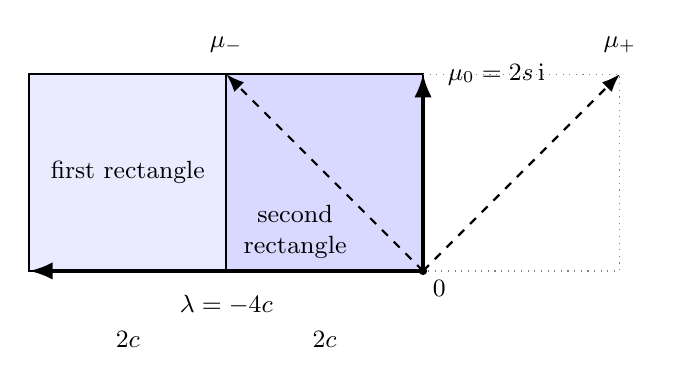
\begin{tikzpicture}[x=1.25cm,y=1.25cm,>=Latex,every node/.style={font=\small}]
\coordinate(O) at (0,0);
\coordinate(L) at (-4,0);
\coordinate(M) at (0,2);
\fill[blue!8] (-4,0) rectangle (-2,2);
\fill[blue!15] (-2,0) rectangle (0,2);
\draw[thick] (-4,0) rectangle (0,2);
\draw[thick] (-2,0)--(-2,2);
\draw[->,very thick] (O)--(L) node[midway,below=5pt] {$\lambda=-4c$};
\draw[->,very thick] (O)--(M) node[right=5pt] {$\mu_0=2s\,\ii$};
\draw[->,thick,dashed] (O)--(-2,2) node[above=4pt] {$\mu_-$};
\draw[->,thick,dashed] (O)--(2,2) node[above=4pt] {$\mu_+$};
\draw[gray,dotted] (0,2)--(2,2)--(2,0)--(0,0);
\node at (-3,1) {first rectangle};
\node[align=center,text width=1.5cm] at (-1.3,.4) {second\\rectangle};
\node at (-3,-.7) {$2c$};
\node at (-1,-.7) {$2c$};
\fill(O) circle(1.5pt);
\node[below right] at(O) {$0$};
\end{tikzpicture}

\caption{The crossing-circle cusp in the original leaf coordinate,
after rotation by $e^{-\pi\ii a}$. Put $s=\sin\pi a$ and
$c=\cos\pi a$. The pure meridian is $2s\,\ii$ and the disk
longitude is $-4c$. Two rectangles of width $2c$ and height $2s$
give one fundamental parallelogram. The dashed vectors are
$\mu_-=\mu_0+\lambda/2$ and $\mu_+=\mu_0-\lambda/2$,
each for its own half-twist partner.}
\label{cg:fig-cusp}
\end{figure}

The adjacent sides of the original rectangle have lengths
$|E-1|=2\sin\pi a$ and $|E+1|=2\cos\pi a$.
The two rectangles of the cusp have total area
$8\sin\pi a\cos\pi a=4\sin2\pi a$. On the other hand
\begin{equation}\label{cg:lattice-area}
 \left|\operatorname{Im}(\overline{\mu_0}\lambda)\right|
       =4\sin2\pi a .
\end{equation}
The two traced closed curves span a sublattice of the actual cusp
lattice; equality of areas makes its index one. Substitution of
either odd meridian leaves the area unchanged, proving the
primitive marking for those collars as well.

Finally $(E+1)/(E-1)=-\ii\cot\pi a$.
Equations \eqref{cg:translations}--\eqref{cg:half-shear} give
\eqref{cg:cusp-shape}, with
$\operatorname{Im}\tau_\eps=2c_\ell/(1+\eps^2c_\ell^2)>0$.
The bound on $c_\ell$ is the imported leaf window
\eqref{cg:leaf-window}. This completes Theorem~\ref{cg:main}.
All main cusps were already included in the horocycle construction;
no additional eigenvalue or deformation hypothesis is required.

\section{Choosing a knot among the main components}
\label{cg:knot}

The construction kept every main component. A finite endpoint
argument produces a one-component choice throughout the stated
grammar.

\begin{proposition}\label{cg:knot-choice}
One can choose pure or odd leaves in every closed expression of
Definition~\ref{cg:grammar} so that its main strands form one
component. Either sign may be used at an odd leaf. Subsequent
full twists preserve that component count.
\end{proposition}
\begin{proof}
Write the three pairings of four cyclically ordered endpoints as
\[
 I=(0,3)(1,2),\qquad U=(0,1)(2,3),\qquad X=(0,2)(1,3).
\]
A pure leaf has pairing $U$, an odd leaf has pairing $X$, and
turn exchanges $I,U$ and fixes $X$. Tracing the two stack
connections gives
\begin{center}
\begin{tabular}{c|ccc}
lower/upper & $I$ & $U$ & $X$\\ \hline
$I$ & $I$ & $U$ & $X$\\
$U$ & $U$ & $U$ and one internal circle & $U$\\
$X$ & $X$ & $U$ & $I$
\end{tabular}
\end{center}
Only $U\cdot U$ creates an internal component.
The base $hh$ has loop-free possibilities $\{I,U\}$.
Put $A=\{I,U\}$, $B=\{I,X\}$, $C=\{U,X\}$,
$D=\{I,U,X\}$. All products, discarding $U\cdot U$, give
\begin{center}
\begin{tabular}{c|ccc}
 & $A$ & $B$ & $C$\\ \hline
$A$ & $A$ & $D$ & $C$\\
$B$ & $D$ & $B$ & $D$\\
$C$ & $C$ & $D$ & $A$
\end{tabular}
\end{center}
Each result contains at least two choices, also if an input
already contains all three. Attaching a leaf is the row or column
$C$. A turn permutes the possibilities. Inductively every completed
box, and the root stack, has at least two loop-free choices.
At least one is $U$ or $X$, whose cylindrical closure is connected;
the closure of $I$ has two components. Backtracking the choices
specifies the required leaves. Both signs have pairing $X$,
and full twists have even endpoint permutation.
\end{proof}

The last assertion concerns connectivity. Theorem~\ref{cg:main}
proves hyperbolicity of the augmented exteriors, retaining the
crossing circles. Hyperbolicity after filling those circles
requires separate deformation and slope arguments.

\section{Dependencies and finite algebra checks}\label{cg:checks}

The variational existence, uniqueness and leaf interval are the
numbered inputs from \cite{Newton} listed in Section~\ref{cg:intro}.
The cell and complement construction, entire face maps, cusp
decoration and primitive marking are proved here.
The ideal-tetrahedron volume formula \eqref{cg:tetra} is classical
background. The references on augmented links and variational
geometry provide context and do not replace the ordered construction.
No quantum asymptotic enters Theorem~\ref{cg:main}.
Corollary~\ref{cg:source-volume} additionally uses the positive
source limit of \cite[Corollary~5.4]{Newton}.

The deterministic program \texttt{check.py} checks rational-function
identities: nine prism maps, turn and closure compatibility, pure
and odd edge returns, and the complete translations
\eqref{cg:translations}. It enumerates the endpoint pairings
independently of the tables in Section~\ref{cg:knot}. Its negative
controls alter a vertex order and an odd meridian. The output
records source hashes. These finite checks support the displayed
algebra; they do not prove convexity, identify a manifold, establish
completeness or supply the stationary-point theorem.

\begin{thebibliography}{9}
\bibitem{Newton}
\emph{Newton coefficients and positive sources for Conway tangles},
companion paper, Definition~2.1, Proposition~5.3,
Corollary~5.4 and Lemma~6.1.
\href{https://sashakolpakov.github.io/murakamis_dream/papers/newton-tangles.pdf}
{Companion PDF}; source: \texttt{papers/newton-tangles/main.tex}.

\bibitem{Milnor}
J.~Milnor, Hyperbolic geometry: the first 150 years,
\emph{Bull.\ Amer.\ Math.\ Soc.\ (N.S.)} \textbf{6} (1982), 9--24.
\href{https://doi.org/10.1090/S0273-0979-1982-14958-8}
{doi:10.1090/S0273-0979-1982-14958-8}.

\bibitem{Purcell}
J.~S.~Purcell, An introduction to fully augmented links,
\emph{Contemp.\ Math.} \textbf{541} (2011), 205--220.
\href{https://users.monash.edu.au/~jpurcell/papers/expos-auglinks.pdf}
{Author's manuscript}.

\bibitem{Rivin}
I.~Rivin, Euclidean structures on simplicial surfaces and hyperbolic
volume, \emph{Ann.\ of Math.} \textbf{139} (1994), 553--580.
\href{https://doi.org/10.2307/2118572}{doi:10.2307/2118572}.
\end{thebibliography}

\end{document}
